\documentclass[../main]{subfiles}
\ifSubfilesClassLoaded{\setcounter{chapter}{6}}{}
\begin{document}

\chapter{Fungsi Hash dan Tanda Tangan Digital}

\begin{subcpmk}
  \item Sub-CPMK 5.1: Mengimplementasikan fungsi hash (MD5, SHA) dan menjelaskan konsep collision
  \item Sub-CPMK 5.2: Menerapkan skema tanda tangan digital (DSA, RSA-Sig) dan memahami struktur sertifikat digital (X.509)
\end{subcpmk}

% ============================================================
% MATERI POKOK
% ============================================================
\section{Sifat Fungsi Hash Kriptografis}

Fungsi hash memetakan input dengan panjang sembarang ke output dengan panjang tetap (misalnya 256 bit) \cite{stallings2017}. Konstruksi Merkle-Damgård menjadi fondasi bagi MD5, SHA-1, SHA-2 \cite{menezes1996}.

Fungsi hash kriptografis harus memenuhi:
\begin{itemize}
  \item \textbf{Preimage resistance}: Dari $h(x)$, sulit mencari $x$
  \item \textbf{Second preimage resistance}: Dari $x$, sulit mencari $x' \neq x$ dengan $h(x') = h(x)$
  \item \textbf{Collision resistance}: Sulit mencari pasangan $(x, x')$ dengan $x \neq x'$ dan $h(x) = h(x')$
\end{itemize}

\textbf{Penggunaan}: Integritas data, penyimpanan password (hash + salt), tanda tangan digital (hash pesan lalu tanda tangan hash) \cite{stallings2017}.

\subsection{Konstruksi Merkle-Damgård}

Konstruksi Merkle-Damgård menggunakan fungsi kompresi collision-resistant dan iterasi blok demi blok \cite{menezes1996}. Dasar bagi MD5, SHA-1, SHA-2. SHA-3 menggunakan konstruksi sponge yang berbeda \cite{stallings2017}.

\subsection{Avalanche Effect}

Perubahan kecil pada input menyebabkan perubahan besar pada output. Setiap bit input mempengaruhi banyak bit output \cite{stallings2017}.

\subsection{Standard Hash Modern}

SHA-2 (SHA-224, SHA-256, SHA-384, SHA-512): standar NIST, aman \cite{stallings2017}. SHA-3 (Keccak): standar alternatif dengan konstruksi sponge; tahan terhadap serangan yang menargetkan Merkle-Damgård \cite{menezes1996}.

\section{Contoh Perhitungan Hash (Simulasi)}

\subsection{Konsep Fungsi Kompresi}

Fungsi hash modern (seperti SHA-256) bekerja dengan memproses pesan dalam blok-blok menggunakan \textbf{fungsi kompresi}. Untuk memahami ini, mari kita lakukan simulasi manual satu langkah fungsi kompresi sederhana.

\textbf{Algoritma Mainan (Toy Hash)}:
\begin{itemize}
  \item \textbf{Input}: Pesan 4-bit ($M$) dan State 4-bit ($H$)
  \item \textbf{Output}: State baru 4-bit ($H'$)
  \item \textbf{Fungsi Kompresi}: $H' = (H \oplus M) + (H \lll 1) \pmod{16}$
\end{itemize}

\subsection{Simulasi Step-by-Step}

\textbf{Pesan}: "A" (ASCII 65 = 0100 0001 biner)
\textbf{IV (Initial Vector)}: 0000

Pesan dibagi menjadi 2 blok 4-bit:
\begin{itemize}
  \item $M_1 = 0100$ (4)
  \item $M_2 = 0001$ (1)
\end{itemize}

\textbf{Langkah 1: Proses Blok 1 ($M_1 = 4$)}
\begin{itemize}
  \item $H_{in} = 0000$ (0)
  \item $H \oplus M = 0000 \oplus 0100 = 0100$ (4)
  \item $H \lll 1 = 0000 \text{ rotasi kiri 1} = 0000$ (0)
  \item $H_{out} = (4 + 0) \pmod{16} = 4$ (0100)
\end{itemize}
State sekarang: $H_1 = 0100$

\textbf{Langkah 2: Proses Blok 2 ($M_2 = 1$)}
\begin{itemize}
  \item $H_{in} = 0100$ (4)
  \item $H \oplus M = 0100 \oplus 0001 = 0101$ (5)
  \item $H \lll 1 = 0100 \text{ rotasi kiri 1} = 1000$ (8)
  \item $H_{out} = (5 + 8) \pmod{16} = 13$ (1101)
\end{itemize}
State sekarang: $H_2 = 1101$ (D dalam heksadesimal)

\textbf{Hash Akhir}: D

\subsection{Efek Avalanche}

Mari ubah 1 bit pesan awal. "A" (0100 0001) $\rightarrow$ "C" (0100 0011).
Perubahan pada blok 2: $M'_2 = 0011$ (3).

\textbf{Langkah 1 (Sama)}: $H_1 = 0100$

\textbf{Langkah 2 (Baru)}:
\begin{itemize}
  \item $H_{in} = 0100$ (4)
  \item $H \oplus M' = 0100 \oplus 0011 = 0111$ (7)
  \item $H \lll 1 = 1000$ (8)
  \item $H_{out} = (7 + 8) \pmod{16} = 15$ (1111)
\end{itemize}
State Akhir: F

Perubahan 1 bit input mengubah output dari D (1101) menjadi F (1111). Meskipun sederhana, ini mengilustrasikan efek avalanche.

\subsection{Struktur Logika SHA-256 Satu Langkah}

SHA-256 jauh lebih kompleks. Satu langkah (step) dari 64 langkah melibatkan:

\[
T_1 = h + \Sigma_1(e) + Ch(e,f,g) + K_t + W_t
\]
\[
T_2 = \Sigma_0(a) + Maj(a,b,c)
\]
\[
h = g, g = f, f = e, e = d + T_1, d = c, c = b, b = a, a = T_1 + T_2
\]

Dimana:
\begin{itemize}
  \item $\Sigma_0, \Sigma_1$: Rotasi dan shift bit (diffusion)
  \item $Ch, Maj$: Fungsi logik non-linear (confusion)
  \item $W_t$: Message schedule (perluasan input)
  \item $K_t$: Konstanta ronde (untuk menghambat analisis)
\end{itemize}

Setiap operasi di atas adalah operasi 32-bit. Kompleksitas ini memastikan bahwa tidak ada jalan pintas matematis untuk membalikkan fungsi hash.

\section{Sistem Kriptografi Merkle-Hellman}

\begin{subcpmk}
  \item Mahasiswa mampu mengimplementasikan prosedur pembangkitan kunci, proses enkripsi, dan proses dekripsi pada sistem Merkle-Hellman Knapsack, serta menganalisis peran pengacakan modular dalam menyembunyikan struktur superincreasing.
\end{subcpmk}

\noindent\textit{Rujukan:} Referensi Knapsack 2026; HAC Bab~8 \cite{hac_online}.

\subsection{Gagasan Utama: Menyembunyikan Struktur}

Kelemahan utama dari barisan superincreasing adalah kemudahannya untuk dipecahkan menggunakan algoritma \textit{greedy}. Oleh karena itu, Ralph Merkle dan Martin Hellman mengusulkan sebuah mekanisme untuk menyembunyikan barisan superincreasing (sebagai kunci privat) menjadi sebuah barisan bilangan bulat acak (sebagai kunci publik) melalui transformasi linear modular.

Kunci publik $P$ tampak seperti barisan acak sehingga penyerang terpaksa menghadapi \textit{Subset Sum Problem} yang NP-complete. Namun, pemilik kunci privat yang mengetahui parameter transformasi dapat mengembalikan $P$ menjadi barisan superincreasing asal, sehingga dekripsi menjadi trivial.

\subsection{Prosedur Operasional Merkle-Hellman}

\subsubsection{Pembangkitan Kunci (Key Generation)}
\begin{enumerate}
    \item \textbf{Memilih Barisan Privat}: Pilih sebuah barisan superincreasing $S = \{s_1, s_2, \dots, s_n\}$.
    \item \textbf{Memilih Parameter Transformasi}: Pilih dua bilangan bulat $m$ dan $q$ sedemikian sehingga:
    \begin{itemize}
        \item $q > \sum_{i=1}^n s_i$ (untuk mencegah overflow saat modulo).
        \item $\gcd(m, q) = 1$ (agar $m$ memiliki invers modulo $q$).
    \end{itemize}
    \item \textbf{Menghitung Kunci Publik}: Hitung setiap elemen kunci publik $p_i$ menggunakan rumus:
    \begin{equation}
      p_i = (s_i \cdot m) \pmod{q}
    \end{equation}
\end{enumerate}
\textbf{Kunci Privat}: $(S, m, q)$ \\
\textbf{Kunci Publik}: $P = \{p_1, p_2, \dots, p_n\}$

\subsubsection{Proses Enkripsi}
Untuk mengenkripsi pesan biner $M = (m_1, m_2, \dots, m_n)$ di mana $m_i \in \{0, 1\}$, pengirim menghitung jumlah terboboti dari kunci publik:
\begin{equation}
  T = \sum_{i=1}^{n} m_i \cdot p_i
\end{equation}
Cipherteks yang dikirimkan adalah nilai skalar $T$.

\subsubsection{Proses Dekripsi}
Penerima menggunakan kunci privat untuk mengembalikan $T$ menjadi bentuk superincreasing $T'$:
\begin{enumerate}
    \item \textbf{Hitung Invers Modular}: Temukan $m^{-1} \pmod{q}$ menggunakan Algoritma Euclidean Diperluas.
    \item \textbf{Transformasi Balik}: Hitung nilai $T'$ sebagai berikut:
    \begin{equation}
      T' = (T \cdot m^{-1}) \pmod{q}
    \end{equation}
    \item \textbf{Ekstraksi Bit}: Karena $T'$ adalah jumlah dari barisan superincreasing $S$, gunakan algoritma \textit{greedy} untuk menentukan bit $m_i$.
\end{enumerate}

\begin{figure}[htbp]
  \centering
  \includegraphics[width=0.8\textwidth]{example-image-a}
  \caption{Alur kerja sistem Merkle-Hellman: Transformasi barisan superincreasing menjadi kunci publik, proses enkripsi melalui penjumlahan subset, dan dekripsi menggunakan invers modular.}
  \label{fig:mh-flow}
\end{figure}

\subsection{Contoh Trace Manual Merkle-Hellman}

Misalkan kita menggunakan parameter berikut:
\begin{itemize}
    \item Barisan privat $S = \{2, 5, 11, 21, 45\}$. (Cek: $2+5+11+21 = 39 < 45 \checkmark$).
    \item Parameter: $m = 7, q = 101$. ($\gcd(7, 101)=1$ dan $101 > 83 \checkmark$).
\end{itemize}

\textbf{1. Pembentukan Kunci Publik $P$}:
\begin{align*}
  p_1 &= (2 \cdot 7) \pmod{101} = 14 \\
  p_2 &= (5 \cdot 7) \pmod{101} = 35 \\
  p_3 &= (11 \cdot 7) \pmod{101} = 77 \\
  p_4 &= (21 \cdot 7) \pmod{101} = 147 \pmod{101} = 46 \\
  p_5 &= (45 \cdot 7) \pmod{101} = 315 \pmod{101} = 12
\end{align*}
Maka $P = \{14, 35, 77, 46, 12\}$.

\textbf{2. Enkripsi Pesan} $M = (1, 0, 1, 0, 1)$:
\[ T = (1 \cdot 14) + (0 \cdot 35) + (1 \cdot 77) + (0 \cdot 46) + (1 \cdot 12) = 14 + 77 + 12 = 103 \]

\textbf{3. Dekripsi}:
\begin{itemize}
    \item Cari $m^{-1} \pmod{101}$: $7 \cdot 29 = 203 = 2 \cdot 101 + 1$. Jadi $m^{-1} = 29$.
    \item Hitung $T' = (103 \cdot 29) \pmod{101} = 2987 \pmod{101} = 58$.
    \item Selesaikan $T' = 58$ dengan $S = \{2, 5, 11, 21, 45\}$ menggunakan algoritma \textit{greedy}:
    \begin{itemize}
        \item $58 \ge 45 \rightarrow$ Ambil 45. Sisa $58-45 = 13$.
        \item $13 \ge 21$ (Tidak)
        \item $13 \ge 11 \rightarrow$ Ambil 11. Sisa $13-11 = 2$.
        \item $2 \ge 5$ (Tidak)
        \item $2 \ge 2 \rightarrow$ Ambil 2. Sisa $2-2 = 0$.
    \end{itemize}
    Hasil bit: $(1, 0, 1, 0, 1)$. (Terbukti!)
\end{itemize}

\subsection{Implementasi dalam Python}

\begin{pycode}
def modInverse(a, m):
    m0, y, x = m, 0, 1
    if m == 1: return 0
    while a > 1:
        q = a // m
        t = m
        m = a % m
        a = t
        y, x = x - q * y, y
    if x < 0: x = x + m0
    return x

def encrypt_knapsack(message, public_key):
    return sum(m_i * p_i for m_i, p_i in zip(message, public_key))

def decrypt_knapsack(ciphertext, private_key, m, q):
    S, m_inv = private_key, modInverse(m, q)
    t_prime = (ciphertext * m_inv) % q

    message = []
    for s in reversed(S):
        if t_prime >= s:
            message.append(1)
            t_prime -= s
        else:
            message.append(0)
    return message[::-1]

# Pengujian
S = [2, 5, 11, 21, 45]
m, q = 7, 101
P = [(s * m) % q for s in S]
msg = [1, 0, 1, 0, 1]
ct = encrypt_knapsack(msg, P)
pt = decrypt_knapsack(ct, S, m, q)
print(f"Msg: {msg} -> CT: {ct} -> PT: {pt}")
\end{pycode}

\begin{aktivitas}
  \item \textbf{Eksperimen Parameter}: Cobalah mengubah nilai $m$ dan $q$ pada implementasi Python di atas. Apa yang terjadi jika $\gcd(m, q) \neq 1$? Mengapa hal ini menyebabkan kegagalan dekripsi?
\end{aktivitas}

\begin{latihan}
  \item Diketahui kunci publik $P = \{15, 27, 51, 95, 187\}$ dan modulus $q=256$. Jika Anda mengetahui bahwa barisan superincreasing asal adalah $S = \{1, 2, 4, 8, 16\}$, tentukan nilai $m$ yang digunakan!
  \item Mengapa pemilihan $q$ harus lebih besar dari jumlah seluruh elemen barisan superincreasing $S$? Jelaskan konsekuensinya jika $q \le \sum s_i$!
  \item Buktikan bahwa jika $S$ adalah barisan superincreasing, maka setiap jumlah subset dari $S$ menghasilkan nilai yang unik!
\end{latihan}

\section{MAC, HMAC, dan Birthday Paradox}

\subsection{Birthday Paradox}

Untuk fungsi hash dengan output $n$ bit, serangan brute-force collision memerlukan sekitar $2^{n/2}$ percobaan karena \textbf{Birthday Paradox} \cite{stallings2017}. Dalam kelompok $\sqrt{2^n} \approx 2^{n/2}$ input acak, probabilitas menemukan collision mendekati 50\%.

Implikasi: hash 128-bit (MD5) memiliki keamanan collision efektif sekitar $2^{64}$; hash 256-bit (SHA-256) sekitar $2^{128}$. Oleh karena itu SHA-256 direkomendasikan untuk keamanan jangka panjang \cite{menezes1996}.

\subsection{MAC (Message Authentication Code)}

MAC memastikan \textbf{integritas dan otentikasi} pesan menggunakan kunci rahasia bersama. MAC$(m, K) = \tau$; verifikasi: hitung ulang MAC dan bandingkan. Berbeda dengan hash biasa, MAC memerlukan kunci—penyerang tanpa kunci tidak dapat memalsukan MAC valid \cite{stallings2017}.

\subsection{HMAC}

HMAC (Hash-based MAC) mengkombinasikan fungsi hash $H$ dengan kunci $K$ \cite{stallings2017}:
\[
\text{HMAC}(K, m) = H\bigl( (K' \oplus \text{opad}) \| H( (K' \oplus \text{ipad}) \| m ) \bigr)
\]
dengan $K'$ adalah kunci yang dipad/dipotong ke ukuran blok hash, opad dan ipad konstanta.

HMAC aman selama hash dasarnya aman. Digunakan untuk autentikasi dalam TLS, API, JWT. Gunakan SHA-256 atau SHA-3 sebagai hash dasar \cite{menezes1996}.
\section{Tanda Tangan Digital Berbasis RSA}

\subsection{Konsep dan Matematika}

Tanda tangan digital memastikan keaslian dan integritas pesan. Alice menandatangani pesan $m$ dengan kunci privatnya. Bob memverifikasi dengan kunci publik Alice. Menurut Wikipedia, tanda tangan digital merupakan salah satu aplikasi paling penting dari kriptografi asimetris, memungkinkan verifikasi otomatis dan non-repudiasi dalam transaksi digital.

Tanda tangan digital RSA secara matematis menggunakan operasi modular yang sama dengan enkripsi RSA. Menurut Wikipedia, untuk membuat tanda tangan, Alice menghitung hash pesan $h = H(m)$, kemudian mengenkripsi hash tersebut dengan kunci privatnya: $s = h^d \bmod n$. Verifikasi dilakukan dengan mendekripsi tanda tangan menggunakan kunci publik dan membandingkan dengan hash ulang: $h' = s^e \bmod n$.

\subsection{Skema RSA-Based}

Alice menghitung $h = H(m)$ (hash pesan), lalu $s = h^d \bmod n$ dengan kunci privat $(d, n)$. Tanda tangan: $s$. Menurut Wikipedia, skema ini disebut "RSA with Appendix" karena menandatangani hash pesan daripada pesan langsung. Ini memungkinkan tanda tangan yang lebih pendek dan efisien untuk pesan besar.

Bob memverifikasi: menghitung $h' = s^e \bmod n$ dengan kunci publik $(e, n)$, lalu $h = H(m)$. Jika $h' = h$, tanda tangan valid. Menurut sumber keamanan, verifikasi ini berhasil karena sifat matematika RSA: $(h^d)^e \equiv h^{ed} \equiv h \pmod{n}$ jika $h = H(m)$ dan $m$ relatif prima terhadap $n$.

\subsection{Standar PKCS dan Padding}

PKCS~\#1 mendefinisikan format dan padding yang aman untuk tanda tangan RSA. Menurut Wikipedia, standar ini dikembangkan oleh RSA Laboratories dan menjadi referensi implementasi tanda tangan digital di seluruh dunia. PKCS~\#1 v1.5 mendefinisikan \texttt{RSASSA-PKCS1-v1\_5} (legacy) dan \texttt{RSASSA-PKCS1-v1\_5} dengan appendix (EMSA).

PKCS~\#1 v2.0 memperkenalkan skema yang lebih modern: RSAES-OAEP untuk enkripsi dan RSASSA-PSS untuk tanda tangan. Menurut Wikipedia, OAEP (Optimal Asymmetric Encryption Padding) menggunakan Mask Generation Function (MGF1) untuk menciptakan padding yang semirandom dan aman terhadap serangan chosen-ciphertext. PSS (Probabilistic Signature Scheme) menggunakan salt acak untuk mencegah serangan terhadap skema tanda tangan deterministik.

\subsection{Implementasi Praktis dengan OpenSSL}

Untuk implementasi tanda tangan digital yang aman, gunakan library OpenSSL dengan EVP API. Menurut Wikipedia, OpenSSL menyediakan implementasi RSA yang telah dioptimasi dan diuji secara ekstensif untuk berbagai skema PKCS. Hindari implementasi manual dari operasi RSA tingkat rendah.

\begin{lstlisting}[style=cstyle]
// Contoh implementasi tanda tangan dengan OpenSSL
EVP_PKEY_CTX *ctx = EVP_PKEY_CTX_new(pkey, NULL);
EVP_PKEY_sign_init(ctx);
EVP_PKEY_CTX_set_rsa_padding(ctx, RSA_PKCS1_PSS_PADDING);
EVP_PKEY_CTX_set_signature_md(ctx, EVP_sha256());
EVP_PKEY_sign(ctx, signature, &siglen, message, message_len);
\end{lstlisting}

OpenSSL EVP API menyediakan interface tingkat tinggi yang aman dan konsisten. Menurut dokumentasi OpenSSL, API ini secara otomatis menggunakan constant-time operations, padding yang aman (PSS), dan validasi input yang komprehensif. Penggunaan EVP sangat direkomendasikan untuk aplikasi produksi karena mengurangi risiko implementasi yang salah.

\subsection{Keamanan Implementasi}

Implementasi tanda tangan digital yang aman harus memperhatikan berbagai aspek:
\begin{itemize}
  \item \textbf{Random Number Generation}: Gunakan CSRNG untuk kunci dan salt.
  \item \textbf{Hash Function}: Gunakan hash yang kuat (SHA-256 atau lebih).
  \item \textbf{Padding}: Selalu gunakan padding yang aman (OAEP, PSS).
  \item \textbf{Side-Channel Protection}: Implementasi constant-time operations.
  \item \textbf{Key Management}: Lindungi kunci privat dengan sangat hati-hati.
\end{itemize}

Keamanan implementasi tanda tangan digital sangat bergantung pada keamanan kunci privat. Menurut sumber keamanan, jika kunci privat RSA dikompromikan, semua tanda tangan yang dibuat dengan kunci tersebut dapat dipalsukan. Oleh karena itu, perlindungan kunci privat menggunakan Hardware Security Modules (HSM) atau secure enclaves sangat penting untuk aplikasi keamanan tinggi.

\subsection{Aplikasi dan Use Cases}

Tanda tangan digital RSA digunakan secara luas dalam berbagai aplikasi:
\begin{itemize}
  \item \textbf{Email Security}: S/MIME untuk email yang ditandatangani.
  \item \textbf{Code Signing}: Menandatangani software dan driver untuk verifikasi integritas.
  \item \textbf{Document Signing}: PDF dan dokumen digital yang ditandatangani.
  \item \textbf{Financial Transactions}: Transaksi perbankan dan pembayaran online.
  \item \textbf{Blockchain}: Transaksi cryptocurrency dan smart contracts.
\end{itemize}

Tanda tangan digital menjadi fondasi bagi banyak sistem keamanan modern. Menurut Wikipedia, penggunaan tanda tangan digital memungkinkan otomatisasi proses verifikasi yang sebelumnya memerlukan intervensi manual. Dalam blockchain, tanda tangan digunakan untuk membuktikan kepemilikan transaksi tanpa memerlukan otoritas terpusat.

\section{Advanced Hash Functions dan Modern Constructions}

\subsection{Evolusi dari Merkle-Damgård ke Sponge Construction}

Hash functions modern telah berevolusi dari Merkle-Damgård construction ke sponge construction yang lebih fleksibel dan aman \cite{bertoni2011}. SHA-3 (Keccak) adalah contoh pertama yang menggunakan sponge construction.

\textbf{Merkle-Damgård Construction}:
\begin{itemize}
  \item Digunakan oleh MD5, SHA-1, SHA-2
  \item Vulnerable terhadap length extension attacks
  \item Fixed output size
\end{itemize}

\textbf{Sponge Construction}:
\begin{itemize}
  \item Digunakan oleh SHA-3, BLAKE2
  \item Resistensi terhadap length extension
  \item Flexible output size
  \item Dapat digunakan untuk hash dan PRF
\end{itemize}

\subsection{SHA-3 (Keccak) dan Sponge Construction}

SHA-3 menggunakan sponge construction dengan fungsi keccak-f yang beroperasi pada state 1600-bit \cite{keccak2015}.

\subsubsection{Sponge Construction Fundamentals}

\begin{figure}[htbp]
  \centering
  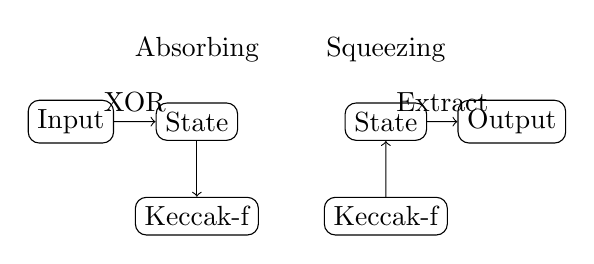
\begin{tikzpicture}[scale=0.8]
    % Absorbing phase
    \node[draw, rounded corners] (state1) at (0,2) {State};
    \node[draw, rounded corners] (input1) at (-2,2) {Input};
    \draw[->] (input1) -- (state1) node[midway, above] {XOR};
    
    % Permutation
    \node[draw, rounded corners] (perm1) at (0,0.5) {Keccak-f};
    \draw[->] (state1) -- (perm1);
    
    % Squeezing phase
    \node[draw, rounded corners] (state2) at (3,2) {State};
    \node[draw, rounded corners] (output1) at (5,2) {Output};
    \draw[->] (state2) -- (output1) node[midway, above] {Extract};
    
    % Permutation
    \node[draw, rounded corners] (perm2) at (3,0.5) {Keccak-f};
    \draw[->] (perm2) -- (state2);
    
    % Labels
    \node[above] at (0,2.8) {Absorbing};
    \node[above] at (3,2.8) {Squeezing};
  \end{tikzpicture}
  \caption{Sponge construction: absorbing dan squeezing phases.}
\end{figure}

\textbf{Operasi Sponge}:
\begin{enumerate}
  \item \textbf{Absorbing}: Input di-XOR ke state, kemudian di-permutasi
  \item \textbf{Squeezing}: Output diekstrak dari state, kemudian di-permutasi
\end{enumerate}

\subsubsection{Keccak-f Permutation}

Keccak-f adalah fungsi permutation yang terdiri dari 24 round, setiap round memiliki 5 langkah:

\begin{lstlisting}[style=cstyle, caption={Keccak-f[1600] Implementation}]
#include <stdint.h>
#include <string.h>

#define STATE_SIZE 200  // 1600 bits = 200 bytes
#define RHO_SIZE 24

typedef struct {
    uint64_t state[25];  // 5x5x64-bit array
} KeccakState;

// Theta step - linear diffusion
void keccak_theta(KeccakState *s) {
    uint64_t C[5], D[5];
    
    // Compute column parity
    for (int x = 0; x < 5; x++) {
        C[x] = s->state[x] ^ s->state[x + 5] ^ s->state[x + 10] ^ 
               s->state[x + 15] ^ s->state[x + 20];
    }
    
    // Compute D
    for (int x = 0; x < 5; x++) {
        D[x] = C[(x + 4) % 5] ^ rotate_left(C[(x + 1) % 5], 1);
    }
    
    // Apply to state
    for (int x = 0; x < 5; x++) {
        for (int y = 0; y < 5; y++) {
            s->state[x + 5*y] ^= D[x];
        }
    }
}

// Rho and Pi steps - bit rotation and permutation
void keccak_rho_pi(KeccakState *s) {
    uint64_t temp[25];
    memcpy(temp, s->state, sizeof(temp));
    
    // Rotation offsets for Keccak-f[1600]
    const int rho_offsets[25] = {
        0, 1, 190, 28, 146, 91, 109, 335, 208, 177,
        113, 200, 230, 228, 132, 154, 41, 229, 90, 240,
        174, 143, 201, 8, 102
    };
    
    // Apply Rho and Pi
    for (int x = 0; x < 5; x++) {
        for (int y = 0; y < 5; y++) {
            int new_x = y;
            int new_y = (2*x + 3*y) % 5;
            int index = x + 5*y;
            int new_index = new_x + 5*new_y;
            
            s->state[new_index] = rotate_left(temp[index], rho_offsets[index]);
        }
    }
}

// Chi step - non-linear substitution
void keccak_chi(KeccakState *s) {
    uint64_t temp[5];
    
    for (int y = 0; y < 5; y++) {
        // Copy row
        for (int x = 0; x < 5; x++) {
            temp[x] = s->state[x + 5*y];
        }
        
        // Apply Chi
        for (int x = 0; x < 5; x++) {
            s->state[x + 5*y] = temp[x] ^ 
                              ((~temp[(x + 1) % 5]) & temp[(x + 2) % 5]);
        }
    }
}

// Iota step - round constant
void keccak_iota(KeccakState *s, int round) {
    // Round constants for Keccak-f[1600]
    const uint64_t RC[24] = {
        0x0000000000000001, 0x0000000000008082, 0x800000000000808A,
        0x8000000080008000, 0x000000000000808B, 0x0000000080000001,
        0x8000000080008081, 0x8000000000008009, 0x000000000000008A,
        0x0000000000000088, 0x0000000080008009, 0x000000008000000A,
        0x000000008000808B, 0x800000000000008B, 0x8000000000008089,
        0x8000000000008003, 0x8000000000008002, 0x8000000000000080,
        0x000000008000000A, 0x800000008000000A, 0x8000000080008081,
        0x8000000000008080, 0x0000000080000002, 0x8000000000000083
    };
    
    s->state[0] ^= RC[round];
}

// Full Keccak-f permutation
void keccak_f(KeccakState *s) {
    for (int round = 0; round < 24; round++) {
        keccak_theta(s);
        keccak_rho_pi(s);
        keccak_chi(s);
        keccak_iota(s, round);
    }
}
\end{lstlisting}

\subsubsection{SHA-3 Implementation}

\begin{lstlisting}[style=cstyle, caption={SHA-3-256 Implementation}]
void sha3_256(const uint8_t *input, size_t input_len, uint8_t *output) {
    KeccakState state;
    memset(&state, 0, sizeof(state));
    
    // Rate and capacity for SHA3-256
    const int rate = 1088;  // 1088 bits = 136 bytes
    const int capacity = 512; // 512 bits = 64 bytes
    const int block_size = rate / 8;
    
    size_t processed = 0;
    
    // Absorbing phase
    while (processed < input_len) {
        // Copy input block to state
        int block_len = (input_len - processed > block_size) ? 
                        block_size : (input_len - processed);
        
        for (int i = 0; i < block_len; i++) {
            ((uint8_t*)state.state)[i] ^= input[processed + i];
        }
        
        // Apply permutation
        keccak_f(&state);
        
        processed += block_len;
    }
    
    // Padding
    uint8_t padding[block_size];
    memset(padding, 0, block_size);
    padding[0] = 0x06;  // SHA-3 padding
    padding[block_size - 1] |= 0x80;
    
    // XOR padding to state
    for (int i = 0; i < block_size; i++) {
        ((uint8_t*)state.state)[i] ^= padding[i];
    }
    
    // Final permutation
    keccak_f(&state);
    
    // Squeezing phase - extract 256-bit hash
    memcpy(output, state.state, 32);
}

// SHA-3 extendable output function
void sha3_xof(const uint8_t *input, size_t input_len, 
              uint8_t *output, size_t output_len) {
    KeccakState state;
    memset(&state, 0, sizeof(state));
    
    // Same absorbing phase as SHA-3
    // ... (same as above)
    
    // Squeezing phase - extract requested output length
    const int rate = 1088;
    const int block_size = rate / 8;
    
    size_t extracted = 0;
    while (extracted < output_len) {
        int copy_len = (output_len - extracted > block_size) ? 
                      block_size : (output_len - extracted);
        
        memcpy(output + extracted, state.state, copy_len);
        extracted += copy_len;
        
        if (extracted < output_len) {
            keccak_f(&state);
        }
    }
}
\end{lstlisting}

\subsection{BLAKE2 dan BLAKE3}

BLAKE2 adalah keluarga hash functions yang dirancang untuk performa tinggi dengan keamanan setara SHA-3 \cite{aumasson2013}. BLAKE3 adalah versi terbaru yang paralel dan tree-based.

\subsubsection{BLAKE2b Implementation}

\begin{lstlisting}[style=cstyle, caption={BLAKE2b Compression Function}]
#include <stdint.h>
#include <string.h>

#define BLAKE2B_BLOCK_SIZE 128
#define BLAKE2B_OUT_SIZE 64

typedef struct {
    uint64_t h[8];
    uint64_t t[2];
    uint64_t f;
} Blake2bState;

// Initialization vectors
static const uint64_t IV[8] = {
    0x6a09e667f3bcc908, 0xbb67ae8584caa73b,
    0x3c6ef372fe94f82b, 0xa54ff53a5f1d36f1,
    0x510e527fade682d1, 0x9b05688c2b3e6c1f,
    0x1f83d9abfb41bd6b, 0x5be0cd19137e2179
};

// G function
static inline uint64_t rotl(uint64_t x, int n) {
    return (x << n) | (x >> (64 - n));
}

static inline void G(uint64_t *v, int a, int b, int c, int d, int x, int y) {
    v[a] = v[a] + v[b] + x;
    v[d] = rotl(v[d] ^ v[a], 16);
    v[c] = v[c] + v[d];
    v[b] = rotl(v[b] ^ v[c], 12);
    v[a] = v[a] + v[b] + y;
    v[d] = rotl(v[d] ^ v[a], 8);
    v[c] = v[c] + v[d];
    v[b] = rotl(v[b] ^ v[c], 7);
}

// Blake2b compression function
void blake2b_compress(Blake2bState *S, const uint8_t *block, 
                     uint64_t t0, uint64_t t1, int last) {
    uint64_t v[16];
    
    // Initialize working vector
    memcpy(v, IV, sizeof(IV));
    memcpy(v + 8, S->h, sizeof(S->h));
    
    v[12] ^= S->t[0];
    v[13] ^= S->t[1];
    v[14] ^= last ? 0xFFFFFFFFFFFFFFFF : 0;
    
    // Load message block
    uint64_t m[16];
    for (int i = 0; i < 16; i++) {
        m[i] = ((uint64_t*)block)[i];
    }
    
    // 12 rounds
    const int sigma[12][16] = {
        {0, 1, 2, 3, 4, 5, 6, 7, 8, 9, 10, 11, 12, 13, 14, 15},
        {14, 10, 4, 8, 9, 15, 13, 6, 1, 12, 0, 2, 11, 7, 5, 3},
        // ... (10 more rounds)
    };
    
    for (int round = 0; round < 12; round++) {
        // Column round
        G(v, 0, 4, 8, 12, m[sigma[round][0]], m[sigma[round][1]]);
        G(v, 1, 5, 9, 13, m[sigma[round][2]], m[sigma[round][3]]);
        G(v, 2, 6, 10, 14, m[sigma[round][4]], m[sigma[round][5]]);
        G(v, 3, 7, 11, 15, m[sigma[round][6]], m[sigma[round][7]]);
        
        // Diagonal round
        G(v, 0, 5, 10, 15, m[sigma[round][8]], m[sigma[round][9]]);
        G(v, 1, 6, 11, 12, m[sigma[round][10]], m[sigma[round][11]]);
        G(v, 2, 7, 8, 13, m[sigma[round][12]], m[sigma[round][13]]);
        G(v, 3, 4, 9, 14, m[sigma[round][14]], m[sigma[round][15]]);
    }
    
    // Update hash state
    for (int i = 0; i < 8; i++) {
        S->h[i] ^= v[i] ^ v[i + 8];
    }
}

// Blake2b hash function
void blake2b(const uint8_t *input, size_t input_len, 
             uint8_t *output, size_t out_len) {
    Blake2bState S;
    
    // Initialize hash state
    memcpy(S.h, IV, sizeof(IV));
    S.h[0] ^= 0x01010000 ^ out_len;  // Output length
    
    S.t[0] = 0;
    S.t[1] = 0;
    S.f = 0;
    
    // Process full blocks
    size_t processed = 0;
    while (processed + BLAKE2B_BLOCK_SIZE <= input_len) {
        blake2b_compress(&S, input + processed, 
                        processed, processed >> 63, 0);
        S.t[0] += BLAKE2B_BLOCK_SIZE;
        if (S.t[0] < BLAKE2B_BLOCK_SIZE) S.t[1]++;
        processed += BLAKE2B_BLOCK_SIZE;
    }
    
    // Process final block
    uint8_t final_block[BLAKE2B_BLOCK_SIZE];
    size_t remaining = input_len - processed;
    memcpy(final_block, input + processed, remaining);
    memset(final_block + remaining, 0, BLAKE2B_BLOCK_SIZE - remaining);
    
    S.t[0] += remaining;
    if (S.t[0] < remaining) S.t[1]++;
    
    blake2b_compress(&S, final_block, S.t[0], S.t[1], 1);
    
    // Extract output
    memcpy(output, S.h, out_len);
}
\end{lstlisting}

\subsubsection{BLAKE3 Tree Hashing}

BLAKE3 menggunakan tree structure untuk parallel processing:

\begin{lstlisting}[style=cstyle, caption={BLAKE3 Tree Structure}]
typedef struct {
    uint8_t hash[32];
    uint64_t len;
    uint8_t flags;
} Blake3Chunk;

// Blake3 chunk processing
void blake3_chunk_hash(const uint8_t *input, size_t len, 
                       uint8_t *output, uint8_t flags) {
    Blake3State state;
    blake3_init(&state, flags);
    
    // Process in 1024-byte chunks
    for (size_t i = 0; i < len; i += 1024) {
        size_t chunk_len = (len - i > 1024) ? 1024 : (len - i);
        blake3_update(&state, input + i, chunk_len);
    }
    
    blake3_finalize(&state, output);
}

// Parallel tree hashing
void blake3_parallel_hash(const uint8_t *input, size_t len, 
                          uint8_t *output, int threads) {
    if (len <= 1024 || threads == 1) {
        blake3_chunk_hash(input, len, output, 0);
        return;
    }
    
    // Split input into chunks
    size_t chunk_size = (len + threads - 1) / threads;
    uint8_t *chunk_hashes = malloc(threads * 32);
    
    // Process chunks in parallel (simplified)
    #pragma omp parallel for
    for (int i = 0; i < threads; i++) {
        size_t start = i * chunk_size;
        size_t end = (start + chunk_size > len) ? len : start + chunk_size;
        
        blake3_chunk_hash(input + start, end - start, 
                         chunk_hashes + i * 32, 
                         (i == threads - 1) ? 1 : 0);  // Last chunk flag
    }
    
    // Combine chunk hashes
    if (threads == 1) {
        memcpy(output, chunk_hashes, 32);
    } else {
        blake3_parallel_hash(chunk_hashes, threads * 32, output, threads / 2);
    }
    
    free(chunk_hashes);
}
\end{lstlisting}

\subsection{HMAC Security Proofs}

HMAC (Hash-based Message Authentication Code) memiliki bukti keamanan formal yang kuat \cite{bellare1996}.

\subsubsection{HMAC Construction}

\begin{lstlisting}[style=cstyle, caption={HMAC Implementation}]
void hmac_sha256(const uint8_t *key, size_t key_len,
                 const uint8_t *message, size_t msg_len,
                 uint8_t *output) {
    uint8_t ipad[64], opad[64];
    uint8_t inner_hash[32], outer_hash[32];
    
    // Prepare key
    uint8_t k[64];
    if (key_len <= 64) {
        memcpy(k, key, key_len);
        memset(k + key_len, 0, 64 - key_len);
    } else {
        sha256(key, key_len, k);
        memset(k + 32, 0, 32);
    }
    
    // Create inner and outer pads
    for (int i = 0; i < 64; i++) {
        ipad[i] = k[i] ^ 0x36;  // Inner pad
        opad[i] = k[i] ^ 0x5c;  // Outer pad
    }
    
    // Inner hash: H(K ^ ipad || message)
    uint8_t inner_input[64 + msg_len];
    memcpy(inner_input, ipad, 64);
    memcpy(inner_input + 64, message, msg_len);
    sha256(inner_input, 64 + msg_len, inner_hash);
    
    // Outer hash: H(K ^ opad || inner_hash)
    uint8_t outer_input[64 + 32];
    memcpy(outer_input, opad, 64);
    memcpy(outer_input + 64, inner_hash, 32);
    sha256(outer_input, 96, outer_hash);
    
    memcpy(output, outer_hash, 32);
}

// HMAC security analysis
void hmac_security_analysis() {
    // HMAC is secure even if:
    // 1. Hash function is a PRF (pseudorandom function)
    // 2. Hash function is collision-resistant
    // 3. Key is properly randomized
    
    // Security bounds:
    // - Forgery probability: <= q^2 / 2^n (q = queries, n = hash output)
    // - Key recovery: Requires 2^n work (same as brute force)
    
    printf("HMAC Security Properties:\n");
    printf("- Pseudorandomness: Yes\n");
    printf("- Collision resistance: Yes (inherited from hash)\n");
    printf("- Key recovery: 2^256 work for HMAC-SHA256\n");
    printf("- Forgery: q^2/2^256 for q queries\n");
}
\end{lstlisting}

\subsection{Performance Comparison}

\begin{table}[htbp]
  \centering
  \small
  \begin{tabular}{lccc}
    \toprule
    Hash Function & Output Size & Throughput (MB/s) & Security Level \\
    \midrule
    SHA-256 & 256 bit & 650 & 128-bit \\
    SHA-3-256 & 256 bit & 300 & 128-bit \\
    BLAKE2b & 256 bit & 1200 & 128-bit \\
    BLAKE3 & 256 bit & 3000 & 128-bit \\
    \bottomrule
  \end{tabular}
  \caption{Perbandingan performa hash functions modern.}
\end{table}

\subsection{Applications and Use Cases}

\textbf{SHA-3 Applications}:
\begin{itemize}
  \item \textbf{Digital Signatures}: DSA, ECDSA dengan SHA-3
  \item \textbf{Password Hashing}: Argon2 menggunakan BLAKE2b
  \item \textbf{Blockchain}: Ethereum menggunakan Keccak-256
  \item \textbf{Random Number Generation}: CSPRNG dengan SHA-3
\end{itemize}

\textbf{BLAKE3 Applications}:
\begin{itemize}
  \item \textbf{File Verification}: Fast integrity checking
  \item \textbf{Version Control}: Git considering BLAKE3
  \item \textbf{Distributed Systems}: Merkle trees for data verification
  \item \textbf{Backup Systems}: Incremental backup verification
\end{itemize}

\begin{catatan}
Advanced hash functions seperti SHA-3 dan BLAKE3 memberikan keamanan dan performa yang superior dibandingkan hash functions klasik. Pemilihan hash function yang tepat tergantung pada kebutuhan aplikasi: keamanan maksimal (SHA-3), performa tinggi (BLAKE2), atau parallel processing (BLAKE3).
\end{catatan}


% ============================================================
% AKTIVITAS PEMBELAJARAN
% ============================================================

\begin{aktivitas}
  \item \textbf{Praktikum}: Gunakan OpenSSL untuk menghitung SHA-256 dari file. Bandingkan hash sebelum dan setelah mengubah satu byte.
  
  \item \textbf{MAC/HMAC}: Hitung HMAC-SHA256 untuk pesan dengan kunci tertentu. Jelaskan perbedaan dengan hash biasa.
  
  \item \textbf{Merancang}: Buat skema tanda tangan digital sederhana dengan RSA dan SHA-256 (paparkan langkah dalam pseudocode).
  
  \item \textbf{Analisis}: Jelaskan Birthday Paradox dan dampaknya pada ukuran hash. Mengapa MD5 tidak aman?
\end{aktivitas}

% ============================================================
% LATIHAN DAN REFLEKSI
% ============================================================

\begin{latihan}
  \item Jelaskan ketiga sifat fungsi hash (preimage, second preimage, collision resistance).
  
  \item Apa perbedaan hash, MAC, dan HMAC? Kapan masing-masing digunakan?
  
  \item Jelaskan Birthday Paradox dan mengapa hash 256-bit memiliki keamanan collision sekitar $2^{128}$.
  
  \item Jelaskan alur tanda tangan digital RSA (RSASSA-PSS) dan verifikasi.
  
  \item Bedakan DSA dan RSA-Sig. Masalah matematika apa yang mendasari masing-masing?
  
  \item Mengapa kita hash pesan sebelum menandatanganinya?
\end{latihan}

% ============================================================
% ASESMEN
% ============================================================

\begin{asesmen}
\textbf{Instrumen Penilaian untuk Sub-CPMK 5.1, 5.2}

\textbf{A. Essay}

\begin{enumerate}
  \item Jelaskan peran fungsi hash dalam tanda tangan digital.
  \item Mengapa SHA-256 lebih direkomendasikan daripada MD5? Apa implikasi Birthday Paradox?
  \item Bedakan MAC dan hash. Mengapa HMAC digunakan untuk autentikasi?
  \item Jelaskan struktur sertifikat X.509 dan chain of trust.
\end{enumerate}

\textbf{B. Implementasi}

Implementasikan dalam C/Python: hitung SHA-256 dan HMAC-SHA256 untuk string input. Gunakan OpenSSL atau library serupa.
\end{asesmen}

% ============================================================
% CHECKLIST KOMPETENSI
% ============================================================

\begin{checklist}
  \item Saya dapat menjelaskan sifat fungsi hash (preimage, second preimage, collision)
  \item Saya memahami Birthday Paradox dan dampaknya pada ukuran hash
  \item Saya dapat menggunakan SHA untuk integritas data dan memahami MAC/HMAC
  \item Saya dapat merancang tanda tangan digital berbasis RSA (RSASSA-PSS)
  \item Saya memahami DSA dan struktur sertifikat X.509
\end{checklist}

% ============================================================
% RANGKUMAN
% ============================================================

\begin{rangkuman}
Bab ini membahas fungsi hash (MD5, SHA-1/256/3), MAC/HMAC, dan tanda tangan digital (RSA-Sig, DSA, ECDSA). Fungsi hash menyediakan integrity, MAC menyediakan integrity+authenticity, dan tanda tangan digital menyediakan non-repudiation.

\textbf{Poin Kunci:}
\begin{itemize}
  \item Fungsi hash: one-way, collision resistance, fixed output
  \item MAC: $MAC_k(m) = H(k \| m)$ untuk integrity dan authenticity
  \item Tanda tangan digital: $Sig = Sign_{priv}(H(m))$, verifikasi dengan kunci publik
  \item Sertifikat X.509: membungkus kunci publik dengan identitas
\end{itemize}

\textbf{Kata Kunci}: \crypt{Fungsi Hash}, \crypt{SHA-256}, \crypt{MAC}, \crypt{HMAC}, \crypt{Tanda Tangan Digital}, \crypt{RSA-Sig}, \crypt{DSA}, \crypt{Sertifikat Digital}
\end{rangkuman}

% ============================================================
% Persiapan untuk Bab Berikutnya
% ============================================================

\begin{transition}
Setelah mempelajari komponen keamanan individual, kita siap untuk memasuki \textbf{Bab VIII: Protokol Keamanan dan Manajemen Kunci}.

Dalam Bab VIII, kita akan melihat bagaimana semua komponen yang telah dipelajari digabungkan dalam protokol praktis:
\begin{itemize}
  \item \textbf{TLS/SSL}: Protokol keamanan internet yang menggabungkan semua konsep
  \item \textbf{PKI}: Infrastruktur untuk distribusi dan verifikasi kunci publik
  \item \textbf{Manajemen Kunci}: Generasi, distribusi, rotasi, dan revokasi kunci
  \item \textbf{RNG}: Generator bilangan acak untuk keamanan kriptografi
\end{itemize}

\textbf{Integrasi Semua Komponen Sebelumnya}:
\begin{itemize}
  \item \textbf{Bab II}: Layanan keamanan — TLS menyediakan semua 4 layanan
  \item \textbf{Bab III}: Matematika — semua operasi dalam protokol
  \item \textbf{Bab IV-V}: Cipher — AES untuk enkripsi data
  \item \textbf{Bab VI}: Kunci publik — RSA untuk pertukaran kunci dan sertifikat
  \item \textbf{Bab VII}: Hash dan MAC — integrity dan authenticity
\end{itemize}

\textbf{TLS sebagai Sistem Lengkap}:
\begin{enumerate}
  \item \textbf{Handshake}: Pertukaran kunci menggunakan RSA atau DH
  \item \textbf{Certificates}: Verifikasi identitas server (dan client)
  \item \textbf{Cipher Suite}: Pilihan algoritma (AES-GCM, SHA-256, dll)
  \item \textbf{Data Protection}: Enkripsi dan MAC untuk semua komunikasi
\end{enumerate}

\textbf{Preview}: Di Bab VIII, kita akan memahami bagaimana HTTPS bekerja — dari handshake awal hingga enkripsi data aplikasi. Kita akan melihat bagaimana sertifikat digital memverifikasi identitas website, bagaimana kunci sesi dihasilkan secara aman, dan bagaimana semua komponen kriptografi bekerja sama untuk menciptakan komunikasi yang aman di internet.

Setelah Bab VIII, Anda akan mengerti bagaimana teori kriptografi diimplementasikan dalam sistem nyata dan siap untuk memahami analisis keamanan di Bab IX serta evaluasi komprehensif di Bab X.
\end{transition}

\ifSubfilesClassLoaded{
  \renewcommand{\bibname}{Daftar Pustaka}
  \bibliographystyle{plain}
  \bibliography{../references}
}{}
\end{document}
